\documentclass[10pt,a4paper]{article}

\usepackage{fontspec}
\usepackage[french]{babel}
\usepackage[margin=1.6cm,top=1.3cm,bottom=1.6cm]{geometry}
\usepackage{amsmath}
\usepackage{array}
\usepackage{booktabs}
\usepackage{tabularx}
\usepackage{graphicx}
\usepackage{xcolor}
\usepackage{enumitem}
\usepackage{titlesec}
\usepackage{microtype}
\usepackage{listings}
\usepackage{tikz}
\usetikzlibrary{arrows.meta,positioning}
\usepackage[hidelinks]{hyperref}

\definecolor{accent}{HTML}{1F4E79}
\definecolor{codebg}{HTML}{F5F7FA}
\titleformat{\section}{\normalsize\bfseries\color{accent}}{\thesection.}{0.4em}{}
\titleformat{\subsection}{\small\bfseries\color{accent}}{\thesubsection}{0.5em}{}
\titlespacing*{\section}{0pt}{6pt}{2pt}
\titlespacing*{\subsection}{0pt}{4pt}{1pt}
\setlist{nosep,leftmargin=1.1em}
\setlist[itemize]{label=\textbullet}
\setlength{\parindent}{0pt}
\setlength{\parskip}{2.5pt}
\setlength{\emergencystretch}{2em}
\pagestyle{plain}

\lstset{
  language=C++,
  basicstyle=\ttfamily\scriptsize,
  backgroundcolor=\color{codebg},
  keywordstyle=\color{accent}\bfseries,
  commentstyle=\color{gray}\itshape,
  morekeywords={noexcept,override,explicit,constexpr,nullptr,delete,default},
  columns=fullflexible,
  keepspaces=true,
  xleftmargin=0.3em,
  framexleftmargin=0.3em,
  aboveskip=0pt,
  belowskip=0pt,
}

\newcommand{\code}[1]{\texttt{#1}}
\newcolumntype{Y}{>{\raggedright\arraybackslash}X}

\begin{document}

\begin{center}
  {\Large\bfseries\color{accent} Compression d'image par DCT et stockage CSR en C++}\\[2pt]
  {\large Conception du code et représentation des données}\\[3pt]
  Romain \textsc{Ben}, Karim \textsc{Zrig} \quad|\quad MAM4 Polytech Nice Sophia, projet C++ \quad|\quad septembre 2026\\[1pt]
  {\small Code source : \url{https://github.com/BnRomain/jpeg-compression}, dossier \code{cpp/}}
\end{center}

\section{Objectif}
En MAM3, nous avions programmé en Python une compression d'image inspirée de JPEG : DCT sur
des blocs $8\times8$, quantification, suppression des hautes fréquences et stockage des
coefficients au format creux CSR avec \code{scipy}, le tout présenté dans une application
Streamlit. Ce projet réécrit l'ensemble en C++20, sans bibliothèque de calcul, sous la forme
d'un programme en ligne de commande, \code{jpeg\_csr}. Le but de la semaine étant d'apprendre
le C++, ce rapport ne revient que brièvement sur l'algorithme. Il explique surtout comment nous
avons représenté chaque objet du problème en C++ (image, bloc, matrice de quantification,
matrice creuse, fichier compressé) et quelles notions du cours ont guidé ces choix. Le code
source, rendu avec ce rapport, est commenté module par module : nous n'en citons ici que de
courts extraits.

\section{L'algorithme en bref}
Pour chaque canal R, G, B et chaque bloc $M$ d'intensités centrées dans $[-128,127]$ :
\[
  D = P\,M\,P^{T}, \qquad P_{k,i} = \frac{C_k}{2}\cos\frac{(2i+1)k\pi}{16}, \qquad
  \hat D_{k,l} = \operatorname{trunc}\!\Big(\frac{D_{k,l}}{\alpha\,Q_{k,l}}\Big),
\]
avec $C_0 = 1/\sqrt{2}$ et $C_k = 1$ sinon. $\hat D_{k,l}$ est ensuite annulé si
$|\hat D_{k,l}| < S$ (seuil) ou si le masque le rejette : le masque carré de la version Python
garde $k,l < F$, le masque triangulaire du sujet $k+l < F$. Les coefficients d'un canal forment
une matrice presque vide, stockée en CSR. La décompression calcule
$\tilde M = P^{T}(\hat D \odot \alpha Q)\,P + 128$, borné à $[0,255]$ ; comme $P$ est
orthogonale, aucune inversion de matrice n'est nécessaire.

\section{Organisation du code}
Le code suit la compilation séparée vue en séance 2 : chaque module a un en-tête dans
\code{include/}, qui documente ses invariants et les exceptions qu'il peut lancer, et ses
définitions dans \code{src/}. Tout est rangé dans l'espace de noms \code{jpeg} ; les fonctions
utilitaires propres à un fichier sont placées dans un espace de noms anonyme, invisible depuis
les autres fichiers. Le \code{Makefile} compile chaque \code{.cpp} en objet avec les options du
cours (\code{-std=c++20 -Wall -Wextra -pedantic}, plus \code{-O2}), recompile dès qu'un en-tête
change et construit deux exécutables à partir des mêmes objets : \code{jpeg\_csr} (avec
\code{main.cpp}) et \code{run\_tests} (avec \code{tests/test\_main.cpp}). La bibliothèque stb,
qui lit et écrit les fichiers PNG et JPEG, n'est incluse que dans \code{image\_io.cpp} : le reste
du programme ne manipule que notre classe \code{Image}. Le schéma suit le trajet des données ;
chaque boîte est un type ou une fonction du code.

\begin{center}
\begin{tikzpicture}[font=\scriptsize, node distance=0.35cm,
    box/.style={draw=accent, fill=accent!8, rounded corners=2pt, align=center, inner sep=3pt},
    flow/.style={-{Stealth[length=1.8mm]}, accent, semithick}]
  \node[box] (in) {fichier PNG/JPEG\\\code{load\_image}};
  \node[box, right=of in] (img) {\code{Image}\\RGB};
  \node[box, right=0.9cm of img, minimum height=0.9cm] (comp) {\code{compress}};
  \node[box, above left=0.15cm and -0.2cm of comp] (q) {\code{QuantizationTable}};
  \node[box, below left=0.15cm and -0.2cm of comp] (m) {\code{const FrequencyMask\&}};
  \node[box, right=0.9cm of comp] (ci) {\code{CompressedImage}\\3 $\times$ \code{SparseMatrix} + $Q$};
  \node[box, right=0.9cm of ci, minimum height=0.9cm] (dec) {\code{decompress}};
  \node[box, right=of dec] (out) {\code{Image}\\\code{save\_png}};
  \node[box, below=0.35cm of ci] (file) {fichier \code{.csr} (\code{save\_compressed}, \code{load\_compressed})};
  \draw[flow] (in) -- (img);
  \draw[flow] (img) -- (comp);
  \draw[flow] (q) -- (comp);
  \draw[flow] (m) -- (comp);
  \draw[flow] (comp) -- (ci);
  \draw[flow] (ci) -- (dec);
  \draw[flow] (dec) -- (out);
  \draw[flow, <->] (ci) -- (file);
\end{tikzpicture}
\end{center}

\section{Représenter les données en C++}

\subsection{L'image : un seul tableau contigu}
\begin{minipage}[t]{0.45\textwidth}
\vspace{0pt}
\begin{lstlisting}
class Image {
public:
    static constexpr std::size_t channels{3};

    Image(std::size_t width, std::size_t height,
          double value = 0.0);

    double& operator()(std::size_t row,
        std::size_t col, std::size_t channel);
    const double& operator()(std::size_t row,
        std::size_t col, std::size_t channel) const;
    // at(): same access, checked
    Image cropped_to_blocks() const;

private:
    std::size_t width_;
    std::size_t height_;
    std::vector<double> pixels_;
};
\end{lstlisting}
\end{minipage}\hfill
\begin{minipage}[t]{0.525\textwidth}
\vspace{0pt}
En Python, l'image était un tableau \code{numpy} de forme $(n_y, n_x, 3)$. Un vecteur de
vecteurs imbriqués aurait demandé une allocation par ligne, sans rien empêcher deux lignes
d'avoir des tailles différentes. Nous rangeons donc les $w\times h\times 3$ intensités dans un
seul \code{std::vector<double>}, ligne par ligne : la valeur \code{(row, col, channel)} est à
l'indice $(\mathit{row}\cdot w + \mathit{col})\cdot 3 + \mathit{channel}$. La mémoire est
contiguë, parcourue dans l'ordre des boucles, et la cohérence entre dimensions et données se
réduit à un invariant : \code{pixels\_.size()} $= w\times h\times 3$, avec des dimensions non
nulles. Le constructeur l'établit, les données sont privées et aucune méthode ne change la
taille. Le type \code{double} reprend le \code{float64} de \code{numpy} et évite des
conversions dans la DCT.
\end{minipage}

\smallskip
L'accès passe par \code{operator()}, surchargé comme l'\code{operator[]} de \code{IntArray}
(TD 4) et de \code{State} (TD 5) : la version non \code{const} renvoie \code{double\&} pour
écrire, la version \code{const} renvoie \code{const double\&} pour lire une image constante,
par exemple dans \code{compress(const Image\&, ...)}. Comme \code{std::vector}, la classe offre
aussi \code{at()}, qui vérifie les bornes et lance \code{std::out\_of\_range} ; les boucles de
calcul utilisent \code{operator()}, sans vérification. Le rognage aux multiples de 8 est une
méthode \code{const} qui renvoie une nouvelle image : l'originale reste intacte.

\subsection{Le bloc \texorpdfstring{$8\times8$}{8x8} et la DCT : une taille fixe, aucune allocation}
Un bloc de pixels, la matrice de passage $P$ et un bloc de coefficients sont tous des matrices
$8\times8$ de réels : un seul type, \code{Matrix8}, les représente. Ses 64 coefficients sont
dans un \code{std::array<double, 64>}, dont la taille est connue à la compilation :
contrairement à \code{std::vector}, aucune allocation dynamique n'a lieu. Ce choix compte, car
une image $512\times512$ contient $3\times64\times64 = 12\,288$ blocs et chaque bloc crée
plusieurs matrices temporaires. Le produit est un opérateur libre
\code{operator*(const Matrix8\&, const Matrix8\&)}, qui n'a besoin que de l'interface publique
et permet d'écrire \code{p\_ * block * p\_transposed\_} comme la formule mathématique.

La classe \code{Dct} calcule $P$ et $P^T$ une seule fois, dans son constructeur, puis les
réutilise pour chaque bloc à travers deux méthodes \code{const}, \code{forward} et
\code{inverse}. Nous y avons rencontré une règle du C++ : les membres sont initialisés dans
l'ordre de leur déclaration dans la classe, et non dans celui de la liste d'initialisation.
\code{p\_} doit donc être déclaré avant \code{p\_transposed\_}, qui est calculé à partir de lui ;
un commentaire le signale dans l'en-tête.

\subsection{La matrice de quantification : un invariant qui fixe un type}
\code{QuantizationTable} encapsule un \code{Matrix8} de diviseurs, avec pour invariant que tous
valent au moins 1. Le constructeur, déclaré \code{explicit} pour interdire la conversion
implicite d'un \code{Matrix8} en table, le vérifie et lance \code{std::invalid\_argument}
sinon ; aucune méthode ne modifie ensuite la table. La condition est écrite \code{!(d >= 1)}
plutôt que \code{d < 1}, pour rejeter aussi une valeur NaN. Cet invariant a une conséquence
directe sur la représentation : un coefficient de DCT vérifie $|D_{k,l}| \leq 8\times128 = 1024$,
donc, divisé par un nombre au moins égal à 1, il tient dans un \code{std::int16\_t}, le type
stocké dans la matrice creuse (l'équivalent de \code{.astype(np.int16)}). Les quatre matrices
étudiées en MAM3 sont des fonctions membres statiques (\code{standard()}, \code{uniform()},
\code{low\_frequencies()}, \code{high\_frequencies()}) qui nomment chaque manière de construire
une table. Le facteur de qualité est une méthode \code{const}, \code{scaled(alpha)}, qui renvoie
une nouvelle table : son constructeur revérifie l'invariant, car $\alpha < 1$ peut produire un
diviseur inférieur à 1.

\subsection{La matrice creuse CSR, écrite à la main}
\begin{minipage}[t]{0.45\textwidth}
\vspace{0pt}
\begin{lstlisting}
class SparseMatrix {
public:
    // from the dense matrix, only read
    SparseMatrix(std::size_t rows, std::size_t cols,
        const std::vector<std::int16_t>& dense);

    // from the arrays read in a .csr file:
    // taken by value, then moved
    SparseMatrix(std::size_t rows, std::size_t cols,
        std::vector<std::int16_t> values,
        std::vector<std::int32_t> column_indices,
        std::vector<std::int32_t> row_pointers);
    ...
private:
    std::size_t rows_;
    std::size_t cols_;
    std::vector<std::int16_t> values_;
    std::vector<std::int32_t> column_indices_;
    std::vector<std::int32_t> row_pointers_;
};
\end{lstlisting}
\end{minipage}\hfill
\begin{minipage}[t]{0.525\textwidth}
\vspace{0pt}
\code{scipy.sparse.csr\_matrix} est remplacée par la classe \code{SparseMatrix}, qui reprend
exactement le format CSR : \code{values\_} contient les \code{nnz} valeurs non nulles, ligne par
ligne, \code{column\_indices\_} la colonne de chacune, et la ligne $i$ occupe les positions
$[\,\mathtt{row\_pointers\_}[i],\ \mathtt{row\_pointers\_}[i+1])$ de ces deux tableaux. Les types
sont ceux de \code{scipy} (valeurs sur 16 bits, indices sur 32 bits), si bien que les tailles
mémoire des deux versions sont directement comparables. Chaque canal est une matrice creuse de
la taille de l'image : le coefficient $(k, l)$ du bloc de coin $(\mathit{top}, \mathit{left})$
est rangé en $(\mathit{top}+k, \mathit{left}+l)$, comme dans la version Python.

L'invariant du format est précis : \code{row\_pointers\_} a $\mathit{rows}+1$ éléments, commence
à 0, croît et se termine à \code{nnz} ; dans une ligne, les colonnes sont strictement croissantes
et dans $[0, \mathit{cols})$ ; aucune valeur stockée n'est nulle.
\end{minipage}

\smallskip
Les deux constructeurs correspondent aux deux usages. Le premier construit le CSR à partir de la
matrice dense des coefficients quantifiés, qu'il ne fait que lire : il la reçoit par
\code{const\&}. Le second reçoit les trois tableaux relus dans un fichier. Il les prend par
valeur puis les déplace dans l'objet avec \code{std::move} (séance 4) ; comme l'appelant lui
transmet ses propres vecteurs avec \code{std::move}, aucun des éléments n'est recopié. Ce
constructeur appelle \code{check\_invariant()}, qui rejette des tableaux incohérents.

\subsection{L'image compressée et le fichier \texorpdfstring{\code{.csr}}{.csr}}
\code{CompressedImage} est une composition (TD 5) : les dimensions, la table de quantification,
indispensable à la décompression, et un \code{std::vector} de trois \code{SparseMatrix}. Son
constructeur vérifie que les dimensions sont des multiples de 8 et que les trois canaux ont la
taille de l'image. Le fichier \code{.csr}, équivalent du \code{.npz} de l'application, contient
une signature, les dimensions, les 64 diviseurs puis, pour chaque canal, \code{nnz} et les trois
tableaux. L'écriture binaire repose sur des fonctions \code{write} et \code{read} surchargées
pour \code{std::uint32\_t}, \code{double} et les vecteurs d'entiers : le compilateur choisit la
version d'après le type de l'argument (séance 2), et \code{reinterpret\_cast} présente chaque
valeur comme une suite d'octets. À la relecture, les dimensions et \code{nnz} sont bornés avant
toute allocation, pour qu'un fichier corrompu ne réserve pas plusieurs gigaoctets ; les
constructeurs de \code{SparseMatrix}, \code{QuantizationTable} et \code{CompressedImage}
revérifient ensuite leurs invariants. Un fichier incohérent est ainsi rejeté par une exception
au lieu de produire une image fausse.

\subsection{Les réglages de la ligne de commande}
Les réglages lus par \code{parse\_options} forment un simple agrégat, \code{struct Options},
dont chaque champ a une valeur par défaut, celle de l'application Python. Nous l'avons laissé en
\code{struct} volontairement : il ne porte pas d'invariant propre, la validité des valeurs étant
contrôlée par les classes qui les utilisent. Les choix discrets (commande, matrice, masque) sont
des \code{enum class} : contrairement à un entier ou à une chaîne, une valeur hors liste ne
compile pas, et \code{-Wall} signale un \code{switch} qui oublierait un cas.

\section{Conception : les notions du cours}

\subsection{Invariants, exceptions et signatures}
Chaque classe suit le schéma du TD 3 : données \code{private}, constructeur qui établit
l'invariant, souvent grâce à une fonction de vérification appelée dans la liste d'initialisation
(comme \code{checked\_capacity} pour \code{IntArray}), et exception sinon. Un objet qui existe
est donc toujours valide, et les fonctions de calcul n'ont rien à revérifier. Toutes les erreurs
(arguments, fichiers, invariants) remontent jusqu'à un unique bloc \code{try}/\code{catch} dans
\code{main}, qui affiche le message et renvoie 1. Les signatures expriment l'intention
(séance 1) : \code{compress} lit ses arguments par \code{const\&} sans les copier,
\code{add\_salt\_and\_pepper(Image\&, ...)} modifie l'image de l'appelant, les petites valeurs
(\code{int}, \code{double}) passent par copie et les accesseurs sont \code{const} et
\code{noexcept}.

\subsection{Ressources : RAII et règle de zéro}
\begin{minipage}[t]{0.45\textwidth}
\vspace{0pt}
\begin{lstlisting}
// image_io.cpp, anonymous namespace
class StbPixels {
public:
    explicit StbPixels(const std::string& path);
    ~StbPixels();   // stbi_image_free(data_)

    StbPixels(const StbPixels&) = delete;
    StbPixels& operator=(const StbPixels&) = delete;
    ...
private:
    int width_{};
    int height_{};
    unsigned char* data_{nullptr};
};
\end{lstlisting}
\end{minipage}\hfill
\begin{minipage}[t]{0.525\textwidth}
\vspace{0pt}
Toutes nos classes composent des types qui gèrent déjà leur mémoire (\code{std::vector},
\code{std::array}) : aucune n'écrit de destructeur ni d'opération de copie ou de déplacement, et
celles que génère le compilateur sont correctes. C'est la règle de zéro (TD 5 et TD de
synthèse) : le programme ne contient aucun \code{new} ni \code{delete}. La seule ressource
manuelle est le tableau de pixels alloué par \code{stbi\_load}, qui doit être libéré par
\code{stbi\_image\_free}.
\end{minipage}

\smallskip
Nous l'avons confié à la classe \code{StbPixels}, sur le modèle de \code{IntArray} (TD 3) et de
la session Gmsh du TD de synthèse : le constructeur acquiert le tableau, le destructeur le libère,
y compris si une exception interrompt \code{load\_image}. La copie est interdite avec
\code{= delete}, car deux objets libéreraient sinon le même tableau, le problème observé au TD 4.
De la même façon, \code{save\_compressed} n'appelle jamais \code{close()} : le destructeur de
\code{std::ofstream} ferme le fichier, même en cas d'erreur.

\subsection{Polymorphisme : un masque choisi à l'exécution}
\begin{minipage}[t]{0.45\textwidth}
\vspace{0pt}
\begin{lstlisting}
class FrequencyMask {
public:
    virtual bool keeps(std::size_t k,
                       std::size_t l) const = 0;
    virtual std::string name() const = 0;
    virtual ~FrequencyMask() = default;
};

// main.cpp: the mask lives on the stack
if (options.mask == MaskKind::triangle) {
    const TriangleMask mask{options.cutoff};
    return compress_with_mask(options, mask);
}
const SquareMask mask{options.cutoff};
return compress_with_mask(options, mask);
\end{lstlisting}
\end{minipage}\hfill
\begin{minipage}[t]{0.525\textwidth}
\vspace{0pt}
La version Python tronquait les hautes fréquences en carré, le sujet de MAM3 en triangle. Plutôt
qu'un paramètre testé dans la boucle de compression, nous avons repris la démarche du TD 6
(\code{ScalarFunction} et \code{midpoint}) : l'interface abstraite \code{FrequencyMask} déclare
\code{keeps(k, l)} virtuelle pure, \code{SquareMask} et \code{TriangleMask} la redéfinissent avec
\code{override}, et le destructeur est virtuel. \code{compress} reçoit un
\code{const FrequencyMask\&} et ne nomme aucune stratégie : ajouter une forme de masque ne
modifie pas son code.
\end{minipage}

\smallskip
Dans \code{main}, le masque demandé est un objet local, construit sur la pile et passé par
référence de base : la référence utilise l'objet sans le posséder ni le copier, ce qui évite
aussi le slicing étudié au TD 5. Le prix est un appel virtuel par coefficient, faible devant les
deux produits matriciels de chaque bloc.

\section{Validation et résultats}
\code{make test} lance 17 fonctions de test à base d'\code{assert} : les tests \code{pytest} de
la version Python (orthogonalité de $P$, rognage, suppression des hautes fréquences, bornes,
conversion CSR), les invariants de chaque classe (un constructeur doit lancer une exception sur
une entrée invalide), l'aller-retour par fichier \code{.csr} et l'analyse de la ligne de
commande. L'intégration continue GitHub les relance sous AddressSanitizer et UBSan, comme en TD,
et mesure la couverture : 91\,\% des lignes de \code{src/} sont exécutées par les tests et la
démonstration. Le script \code{compare\_with\_python.py} compresse la même image avec les deux
versions : 786\,407 coefficients sur 786\,432 sont identiques, avec autant de non nuls. Les 25
autres diffèrent de 1 à cause d'un arrondi flottant côté Python, où l'image passe par $/255$ puis
$\times255$ : $D/Q$ y vaut par exemple $23{,}999\,999\,999\,999\,996$ au lieu de 24, et la
troncature donne 23.

\begin{center}
\begin{minipage}[c]{0.49\textwidth}
{\small
\begin{tabular}{@{}lrrrr@{}}
  \toprule
  Réglage & Conserv. & Erreur $L^2$ & CSR & Gain \\
  \midrule
  $\alpha = 1$ (Python) & 5,79\,\% & 5,43\,\% & 273\,Ko & 22,5 \\
  $\alpha = 5$ & 2,15\,\% & 11,29\,\% & 105\,Ko & 58,5 \\
  $\alpha = 20$ & 0,64\,\% & 32,95\,\% & 35\,Ko & 174,0 \\
  $Q$ uniforme (100) & 1,65\,\% & 13,85\,\% & 82\,Ko & 75,1 \\
  triangle $F=2$ & 2,91\,\% & 11,41\,\% & 140\,Ko & 43,8 \\
  \bottomrule
\end{tabular}}
\end{minipage}\hfill
\begin{minipage}[c]{0.49\textwidth}
  \centering
  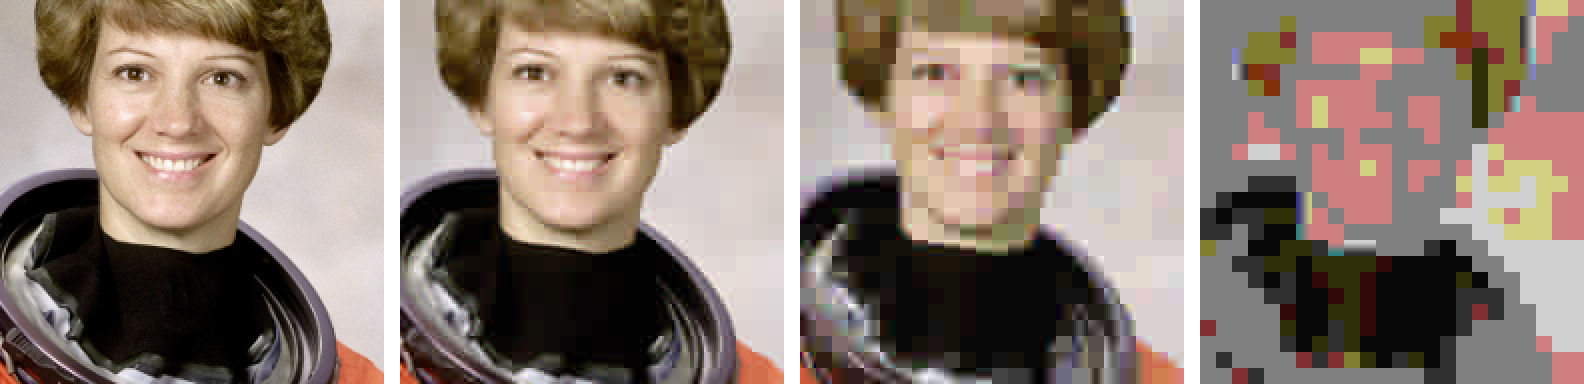
\includegraphics[width=\textwidth]{figures/alpha.png}\\[1pt]
  {\scriptsize originale, puis $\alpha = 1$, $5$ et $20$ (zoom)}
\end{minipage}
\end{center}

Image \code{astronaut.png} ($512\times512$, 6\,144\,Ko en \code{float64}), seuil $S=2$, masque
carré $F=6$ sauf mention contraire ; le gain est le rapport entre la taille dense et la taille
CSR. Comme en MAM3, $\alpha$ règle le compromis entre taux et qualité. Avec 5\,\% de bruit poivre
et sel, l'erreur par rapport à l'image pure passe de 24,0\,\% à 11,3\,\% après compression avec
un masque triangulaire $F=4$ : la troncature agit comme un filtre passe-bas. Compression et
décompression prennent 50\,ms en C++ contre 543\,ms en Python sur la même machine, soit un
facteur 11 : les boucles sont compilées en \code{-O2} et \code{Matrix8} n'alloue rien, là où
\code{numpy} est appelé bloc par bloc.

\section{Difficultés rencontrées}
\begin{itemize}
  \item \textbf{Faire confiance à une bibliothèque C.} L'analyse CodeQL de GitHub a signalé dans stb
    des multiplications d'\code{int} qui calculent des tailles de tampons et peuvent déborder. Nous
    ne compilons que les décodeurs PNG, JPEG et BMP, ces calculs ont été refaits en
    \code{std::size\_t} et les images sont limitées à 16\,384 pixels de côté. Cette limite existe à
    deux endroits, la macro de stb et la constante \code{Image::max\_dimension} : un
    \code{static\_assert} vérifie à la compilation qu'elles restent égales.
  \item \textbf{Les entiers ont une taille.} Les indices CSR sont des \code{int32}, comme dans
    \code{scipy} : le constructeur de \code{SparseMatrix} vérifie que la matrice reste indexable
    sur 32 bits avant toute conversion. Les passages entre \code{int}, \code{std::size\_t} et
    \code{double} sont écrits avec \code{static\_cast}, pour que chaque changement de type se voie
    à la lecture.
  \item \textbf{Garder un niveau d'avertissement élevé.} Compilés avec
    \code{-Wall -Wextra -pedantic}, les en-têtes de stb produisaient des avertissements qui
    noyaient les nôtres : les inclure avec \code{-isystem} les fait taire sans baisser notre niveau
    d'exigence.
  \item \textbf{Un exécutable portable sous Windows.} Un programme compilé avec MinGW dépend de
    bibliothèques partagées que d'autres logiciels (Git, MATLAB) installent dans d'autres versions :
    l'édition de liens statique (\code{-static}) le rend indépendant du \code{PATH}.
  \item \textbf{Vérifier un portage.} Le script de comparaison confronte les 786\,432 coefficients
    un à un plutôt que les images reconstruites, ce qui a permis d'isoler les 25 écarts et de
    remonter à leur cause, un arrondi flottant côté Python.
\end{itemize}

\section{Bilan : ce que le projet nous a appris}
Réécrire un programme que nous connaissions nous a permis de nous concentrer sur le C++ lui-même.
Trois idées ressortent.
\begin{itemize}
  \item \textbf{Le type porte l'information.} En Python, rien n'empêchait une image de dimensions
    quelconques ou un coefficient hors de l'\code{int16} ; en C++, ces hypothèses sont devenues des
    invariants vérifiés une fois, à la construction, et des types choisis en conséquence.
  \item \textbf{Chaque copie se voit.} Choisir entre \code{T}, \code{T\&} et \code{const T\&},
    entre \code{std::array} et \code{std::vector}, ou déplacer plutôt que copier, oblige à savoir
    ce que coûte chaque ligne, ce que \code{numpy} nous cachait.
  \item \textbf{La durée de vie structure le code.} RAII et règle de zéro suppriment la gestion
    mémoire manuelle : la seule ressource brute est enfermée dans une classe de quelques lignes.
\end{itemize}
\textbf{Limites et pistes.} Le fichier \code{.csr} n'est pas un vrai JPEG : il manque le parcours
zigzag et le codage entropique (RLE, Huffman), et l'espace YCbCr permettrait de sous-échantillonner
la chrominance. Côté C++, les pointeurs intelligents, annoncés pour la suite du cours,
permettraient de conserver plusieurs masques polymorphes dans un même conteneur.

\end{document}
